\documentclass[Softwaredesign/Softwaredesign_main.tex]{subfiles}

\usepackage{listings}


\begin{document}
\section{Implementering af RPI\_IF}
Denne klasse består kun af tre funktioner. den ene hedder sendCupStatus(). Denne funktion har til formål at sende cupstatus tilbage til rpi'en, når denne ændres. Denne funktion kan ses nedenfor.
\begin{lstlisting}
void sendCupStatus(uint8_t status)
{
    resetReadBuffer();
    readBuffer[0] = status;
    I2C_SlaveClearReadBuf();
    Interrupt_Write(0);
    CyDelay(1);
    Interrupt_Write(1);
}
\end{lstlisting}
I denne funktion lægges den opdaterede cupstatus over i readbufferen. Herefter kaldes funktionen I2C\_SlaveClearReadBuf(), hvor interrupt benet bliver trukket lavt lige efter. Dette skyldes at rpi'en skal bruge et interrupt for at vide, hvornår den skal læse fra PSoC'en. Efter at interupt benet er trukket lavt, så vil,der være et lille delay for at være sikker på at interruptet registres af rpi'en. Herefter vil interrupt benet igen trækkes højt, så rpi'en igen er klar til at et interrupt modtages. 

Den anden funktion, der er vær at tale om er funktionen RPI\_IF\_handledata(). Denne funktion har til formål at læse fra writebufferem hver gang, der sendes noget til PSoc'en. I et switch statement vil der tjekkes for hvilken besked, der er sendt fra rpi'en og alt afhængig af beskedens indhold,så vil der ske noget forskelligt. Hvis den første byte af beskeden består af en hex værdi fra 0x0A til 0x0E, så vil kun denne byte læses. Disse fem værdier ses ikke i funktion men er defineret ved hjælp af preprocessor makroen #define. De fem makroer ses nedenfor.
\begin{lstlisting}
#define IDLE_DATA 0x0A
#define STARTING_DATA 0x0B
#define PLAYING_DATA 0x0C
#define LOST_DATA 0x0D
#define WON_DATA 0x0E
\end{lstlisting}

Disse fem værdier svarer hver til en af de fem states PSoC'en kan være i. I switch statement vil funktionen setState() blive kaldt i det tilfælde hvor den sendte værdi svarer til en af de fem prædefinerede makroer. Denne funktion er en del af gamecontroller klassen. Udover disse fem states kan en farve besked også sendes til PSoC'en. Denne besked er til forskel fem bytes lang. Selve protocollen for denne besked ses i grænseflade afsnittet. De første to bytes sendt er også defineret med en makro, hvilket ses nedenfor. 
\begin{lstlisting}
#define COLOR_MSG 0x21
#define OPPONENT_COLOR 0x02
#define OWN_COLOR 0x01
\end{lstlisting}
COLOR\_MSG er den første byte, hvor OPPONENT\_COLOR og OWN\_COLOR kan være den næste byte, som er forskellig alt efter om det er playerside sidens egen farve der modtages eller modstanderens. I switch statement vil, der i tilfældet hvor COLOR\_MSG er den besked der bliver er sendt gå ind i dens case i switch statement. Her vil være der være et if statement, som styrer, hvilken farve der skal ændres OPPONENT\_COLOR eller OWN\_COLOR. For en af de to vil der udfra farvekoden sendt, som de tre sidste bytes, laves en  color\_t klasse, som bliver sendt videre som argument til enten funktionen setMyColor eller setOpponentColor i gamecontroller klassen. Til aler sidst i funktionen vil funktionen I2C\_Slave\_clear\_Buf() klades for at buffer pointeren peger på det første element i bufferen igen.
\begin{figure}[H]
    \centering
    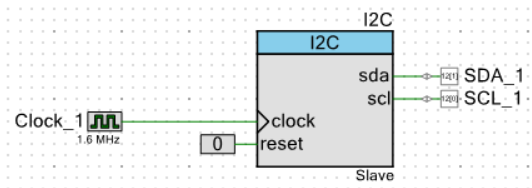
\includegraphics[width=1\textwidth]{Softwaredesign/RPI_IF/graphics/i2c_enhed.PNG}
    \caption{i2c enheden brugt i PSoC}
    \label{fig:i2c_enhed}
\end{figure}
Slave enheden, der bruges i PSoC projektet og som ses i figur \ref{fig:i2c_enhed} er meget let at bruge. Den kræver dog lidt opsætning. Dette gøres i en funktion kaldet RPI\_IF\_init(), som vi laver. Funktionen er vist nedenunder.
\begin{lstlisting}
uint8_t readBuffer[256];
uint8_t writeBuffer[256];
void RPI_IF_init()
{
    I2C_Start();
    I2C_EnableInt();
    
    
    I2C_SlaveInitReadBuf((uint8_t*)readBuffer,255);
    I2C_SlaveInitWriteBuf((uint8_t*)writeBuffer,255);
    
    resetReadBuffer();

}
\end{lstlisting}
Som med alle enheder i PSoC skal den startes ved at bruge funktionen I2C\_Start(). Derefter bliver de indbyggede interrupts i I2C enheden enabled, da enheden, som også forklaret i design afsnittet, bruger interrupts til at opdatere readbufferen efter, at en i2c besked er modtaget fra rpi'en. Til sidst bliver både read og write bufferen initialiseret ved hjælp af endnu en indbygget funktion(funktion, der følger med enhederne i PSoC kataloget), som er henholdsvis I2C\_SlaveInitReadBuf() og I2C\_SlaveInitWriteBuf(). 

\end{document}